%iffalse
\documentclass[journal]{IEEEtran}
\usepackage[a5paper, margin=10mm]{geometry}
%\usepackage{lmodern} % Ensure lmodern is loaded for pdflatex
\usepackage{tfrupee} % Include tfrupee package


\setlength{\headheight}{1cm} % Set the height of the header box
\setlength{\headsep}{0mm}     % Set the distance between the header box and the top of the text


%\usepackage[a5paper, top=10mm, bottom=10mm, left=10mm, right=10mm]{geometry}

%
\setlength{\intextsep}{10pt} % Space between text and floats

\makeindex


\usepackage{cite}
\usepackage{amsmath,amssymb,amsfonts,amsthm}
\usepackage{algorithmic}
\usepackage{graphicx}
\usepackage{textcomp}
\usepackage{xcolor}
\usepackage{txfonts}
\usepackage{listings}
\usepackage{enumitem}
\usepackage{mathtools}
\usepackage{gensymb}
\usepackage{comment}
\usepackage[breaklinks=true]{hyperref}
\usepackage{tkz-euclide} 
\usepackage{listings}
\usepackage{multicol}
\usepackage{xparse}
\usepackage{gvv}
%\def\inputGnumericTable{}                                 
\usepackage[latin1]{inputenc}                                
\usepackage{color}                                            
\usepackage{array}                                            
\usepackage{longtable}                                       
\usepackage{calc}                                             
\usepackage{multirow}                                         
\usepackage{hhline}                                           
\usepackage{ifthen}                                               
\usepackage{lscape}
\usepackage{tabularx}
\usepackage{array}
\usepackage{float}


\newtheorem{theorem}{Theorem}[section]
\newtheorem{problem}{Problem}
\newtheorem{proposition}{Proposition}[section]
\newtheorem{lemma}{Lemma}[section]
\newtheorem{corollary}[theorem]{Corollary}
\newtheorem{example}{Example}[section]
\newtheorem{definition}[problem]{Definition}
\newcommand{\BEQA}{\begin{eqnarray}}
\newcommand{\EEQA}{\end{eqnarray}}

\theoremstyle{remark}


\begin{document}
\bibliographystyle{IEEEtran}
\onecolumn

\title{JEE MAINS 6 Sept 2020 Shift-1}
\author{ee24btech11015 - Dhawal}
\maketitle

\renewcommand{\thefigure}{\theenumi}
\renewcommand{\thetable}{\theenumi}

\begin{enumerate}
	\item The region represented by $\cbrak{ z = x+ \iota y  \in C : z - \text{Re} \brak{z} \leq 1}$ is also given by the inequality $: \cbrak{z = x + \iota y \in C : z -\text{Re} \brak{z} \leq 1}$

\begin{multicols}{4}
\begin{enumerate}
\item $y^2 \leq 2\brak{x + \frac{1}{2}}$
\item $y^2 \leq x + \frac{1}{2}$
\item $y^2 \leq 2\brak{x + 1}$
\item $y^2 \leq x + 1$
\end{enumerate}
\end{multicols}

\item  The negation of the Boolean expression $p \lor (\sim p \land q)$ is equivalent to :

\begin{multicols}{4}
\begin{enumerate}
\item $\sim p \lor  \sim q$
\item $\sim p \lor q$
\item $\sim p \land \sim q$
\item $p \land \sim q$
\end{enumerate}
\end{multicols}

\item  The general solution of the differential equation $\sqrt{1+x^2+y^2+x^2y^2}+xy\brak{\frac{dy}{dx}} = 0$ (where C is a constant of integration)
\begin{enumerate}
\item $\sqrt{1 + y^2} + \sqrt{1 + x^2} = \frac{1}{2} \log_e \brak{ \frac{\sqrt{1 + x^2} - 1}{\sqrt{1 + x^2} + 1} } + c $
\item $\sqrt{1 + y^2} - \sqrt{1 + x^2} = \frac{1}{2} \log_e \brak{ \frac{\sqrt{1 + x^2} - 1}{\sqrt{1 + x^2} + 1} } + c $
\item $\sqrt{1 + y^2} + \sqrt{1 + x^2} = \frac{1}{2} \log_e \brak{ \frac{\sqrt{1 + x^2} + 1}{\sqrt{1 + x^2} - 1} } + c $
\item $\sqrt{1 + y^2} - \sqrt{1 + x^2} = \frac{1}{2} \log_e \brak{ \frac{\sqrt{1 + x^2} + 1}{\sqrt{1 + x^2} - 1} } + c $
\end{enumerate}


\item  Let $L_1$ be a tangent to the parabola $y^2 = 4 \brak{x+1}$and $L_2$ be a tangent to the parabola $y^2 = 8\brak{x+2}$ such that $L_1$ and $L_2$ intersect at right angles. Then $L_1$ and $L_2$ meet on the straight line:

\begin{multicols}{4}
\begin{enumerate}
\item $x+2y = 0$
\item $ x+2 = 0$
\item $ 2x+1 = 0$
\item $x+3 = 0$
\end{enumerate}
\end{multicols}

\item  The area (in sq. units) of the region A = \cbrak{\brak{x, y}: \abs{x}+\abs{y} \leq 1, 2y^2\geq \abs{x}}

\begin{figure}[h] 
    \centering
    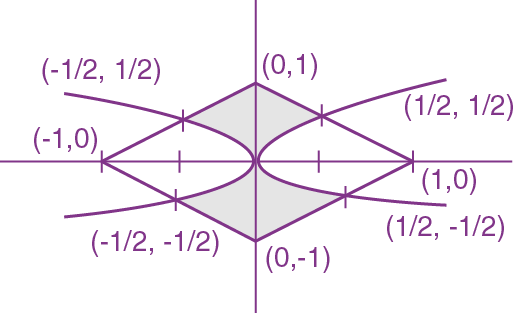
\includegraphics[width=0.5\textwidth]{figure/5.png}
\end{figure}

\begin{multicols}{4}
\begin{enumerate}
\item $\frac{1}{6}$
\item $\frac{5}{6}$
\item $\frac{1}{3}$
\item $\frac{7}{6}$
\end{enumerate}
\end{multicols}

\item  The shortest distance between the lines $\frac{x - 1}{0} = \frac{y + 1}{-1} = \frac{z}{1} \text{ and } x+y+z+1 = 0, 2x-y+z+3 = 0$ is :

\begin{multicols}{4}
\begin{enumerate}
\item $1$
\item $\frac{1}{\sqrt{2}}$
\item $\frac{1}{\sqrt{3}}$
\item $\frac{1}{2}$
\end{enumerate}
\end{multicols}

\item  Let $a, b, c, d \text{ and } p$ be any non zero distinct real numbers such that $\brak{a^2+b^2+c^2}p^2-2\brak{ab+bc+cd}p +\brak{b^2 +c^2+d^2} = 0$. Then:



\begin{multicols}{2}
\begin{enumerate}
\item $a, c, p$ are in G.P.
\item $a, b, c, d$ are in G.P.
\item $ a, b, c, d$ are in A.P.
\item $a, c, p$ are in A.P.
\end{enumerate}
\end{multicols}

\item  Two families with three members each and one family with four members are to be seated in a row. In how many ways can they be seated so that the same family members are not separated?

\begin{multicols}{4}
\begin{enumerate}
\item $(2!) (3!) (4!)$
\item $(3!)^3 (4!)$
\item $ (3!)(4!)^3$
\item $(3!)^2 (4!)$
\end{enumerate}
\end{multicols}

\item  The values of $\lambda$ and $\mu$ for which the system of linear equations\\
$x+y+z = 2$\\
$x+2y+3z = 5$\\
$x+3y+\lambda z = \mu$\\
has infinitely many solutions are, respectively:

\begin{multicols}{4}
\begin{enumerate}
\item $6 \text{ and } 8$
\item $5 \text{ and } 8$
\item $5 \text{ and } 7$
\item $4 \text{ and } 9$
\end{enumerate}
\end{multicols}

\item  Let $m$ and $M$ be respectively the minimum and maximum values of 
\begin{align*}
    \mydet{{\cos}^2x && 1+{\sin}^2x && \sin2x \\1+{\cos}^2x && {\sin}^2x && \sin2x \\ {\cos}^2x && {\sin}^2x && 1+\sin2x}
\end{align*}
Then the ordered pair $(m, M)$ is equal to:
\begin{multicols}{4}
\begin{enumerate}
\item $(-3, -1)$
\item $(-4, -1)$
\item $(1, 3)$
\item $(-3, 3)$
\end{enumerate}
\end{multicols}

\item  A ray of light coming from the point $\myvec{2\\ 2\sqrt{3}}$ is incident at an angle $30\degree$ on the line $x = 1$ at the point $\vec{A}$. The ray gets reflected on the line $x = 1$ and meets x-axis at the point $\vec{B}$. Then, the line AB passes through the point:

\begin{multicols}{4}
\begin{enumerate}
\item $\myvec{4 \\ -\sqrt{3}}$
\item $\myvec{3 \\ -\frac{1}{\sqrt{3}}}$
\item $\myvec{3 \\ -\sqrt{3}}$
\item $\myvec{4 \\ -\frac{\sqrt{3}}{2}}$
\end{enumerate}
\end{multicols}

\item Out of 11 consecutive natural numbers if three numbers are selected at random (without repetition), then the probability that they are in A.P. with positive common difference, is: 

\begin{multicols}{4}
\begin{enumerate}
\item $\frac{10}{99}$
\item $\frac{5}{33}$
\item $\frac{15}{101}$
\item $\frac{5}{101}$
\end{enumerate}
\end{multicols}

\item  If $f(x + y) = f(x) f(y)$ and $\sum_{x=1}^{\infty} f(x) = 2$,\\
$x, y \in $N, where N is the set of all natural number, then the value of $\frac{f(4)}{f(2)}$ is:


\begin{multicols}{4}
\begin{enumerate}
\item $\frac{2}{3}$
\item $\frac{1}{9}$
\item $\frac{1}{3}$
\item $\frac{4}{9}$
\end{enumerate}
\end{multicols}

\item  If $\cbrak{p}$ denotes the fractional part of the number $p$, then $\cbrak{\frac{3^{200}}{8}}$ is equal to:

\begin{multicols}{4}
\begin{enumerate}
\item $\frac{5}{8}$
\item $\frac{1}{8}$
\item $\frac{7}{8}$
\item $\frac{3}{8}$
\end{enumerate}
\end{multicols}

\item  Which of the following points lies on the locus of the foot of perpendicular drawn upon any tangent to the ellipse $\brak{\frac{x^2}{4}}+\brak{\frac{y^2}{2}} = 1$ from any of its foci ?



\begin{multicols}{4}
\begin{enumerate}
\item $\myvec{-1 \\ -\sqrt{3}}$
\item $\myvec{-2 \\ -\sqrt{3}}$
\item $\myvec{-1 \\ -\sqrt{2}}$
\item $\myvec{1 \\ 2}$
\end{enumerate}
\end{multicols}

\begin{figure}[h] 
    \centering
    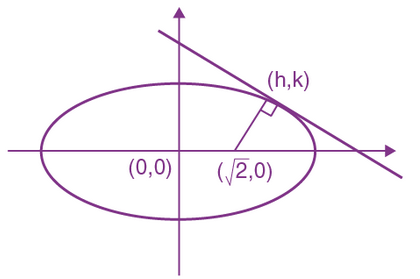
\includegraphics[width=0.5\textwidth]{figure/15.png}
\end{figure}

\end{enumerate}


\end{document}

